% experiments.tex

\chapter{Experiments}
\label{chapter:ch5}
We will now describe our experimental setup in detail, report our findings, and evaluate the experimental results.
Afterward, we will briefly discuss the relevance and impact based on the empirical results.

We are specifically going to investigate the following questions:
\begin{itemize}
    \item Do local models benefit from aggregation?
    \item How do aggregation methods compare to each other? 
    \item Do additional parameter samples affect the aggregate?
    \item How do aggregates perform when compared to the baseline?
\end{itemize}
We evaluated and collected the performance of local models, aggregates, and baseline using the average likelihood, accuracy score, and F1-score relative to the baseline scores. 
Moreover, we continuously monitored the performance of the local and aggregate model to record accuracy and likelihood in every round, with an increasing number of samples.
We then trained a new model on each distributed learner using the extended data set.
To achieve this, we precomputed the number of samples required to satisfy the Hoefding bound. 
Let $n_{\max}$ be the number of samples required.
We then divided the interval between zero and $n_{\max}$ into an arbitrary amount of elements, e.g., fifteen $[10,20,30, \ldots, 150]$ for $n_{\max} = 150$. 
Then for each round, we trained the distributed learners using that amount of samples while aggregating and evaluating the models.
 
We conducted experiments using five different aggregation methods and three covariance matrix sampling variants, while also testing the aggregation without additional parameter vector sampling.
Additionally, we trained models on distributed learners without regularization and with $l2$ regularization.
Operations that involve random events such as sampling or index shuffling were performed using a seeded random state.

The direct comparison of our results is difficult as not much work specifically on aggregating canonical exponential family models has been done. Han and Liu~\cite{han2016bootstrap} considered aggregation on Gaussian mixture models, while Kamp et al. \cite{kamp2017effective} performed experiments using classifier ensembles.
Moreover, the metrics used to compare and evaluate results vary greatly, such that direct comparison is difficult.
Here, we compare our results to integer exponential family models investigated by Piatkowski~\cite{piatkowski2018exponential} obtained by computing the arithmetic mean over a set of distributed learners. 
Integer Markov random fields restrict the solution space of $\vect{\theta}$ to integer values, which in practice is an approximation of the real-valued solution.
However, the aggregate itself does not necessarily need to be an integer model.

We begin the evaluation by first introducing the experimental setup in \autoref{sec:setup}, where we provide an overview of the data sets and detailed data processing steps used.
We then present the experiment framework and evaluation metrics in \autoref{sec:experiments} and \autoref{sec:evaluation}.
Finally, in \autoref{sec:results}, we present, evaluate, and discuss the results.

\section{Data}
\label{sec:setup}

We used three benchmark datasets from the UCI machine learning repository: SUSY~\cite{baldi2014searching}, Covertype~\cite{blackard2000comparison} and Dota2~\cite{tridgell2016dota2} to evaluate the aggregation methods.


We discretized the numerical features containing more than $q$ unique values into their $q=10$ quantiles to obtain comparable results.
Ideally, we determine the interval ranges and number of buckets before the discretization, where the intervals are then based on the total range of each feature.
However, this is usually not the case, i.e., newly observed data from some feature $\mathcal{D}_{\cdot i}$ may contain values outside of the feature range observed in the training data. 
We then observe values exceeding the original range, that is, $\sup(\hat{\vect{X}}_i) > \sup(\vect{X}_i) $ or  $\inf(\hat{\vect{X}}_i) < \inf(\vect{X}_i) $.
We added two additional bins, where samples outside the original range were assigned.
Samples above or below the original range of $\mathcal{D}_{\cdot i}$ were then mapped to buckets $0$ or $q+1$, respectively.

Additionally, we used cross-validation for global models. 
For the distributed learners, we partitioned the training portion of each split further into $k$ equal-sized sets, where $k$ is the number of learners.

The independence structures were estimated using the Chow-Liu algorithm and can be found in Appendix~\ref{sec:apdx:struc}.
Since the structure was re-estimated for each experiment, the structures vary slightly.
The structures were generated on a holdout set of $n=10000$ samples before creating the cross-validation splits.
The holdout set was discretized separately, based on the ranges observed in the holdout set only.
We then discretized the training data and, based on the training data quantiles, the test data as well.

We used three real-world data sets for the experiments and evaluations. 

Each data set is based on a classification task, with two tasks being a binary classification and one multi-class classification.

\paragraph*{Dota2}
The Dota2 data set contains game results of roughly $n=100.000$ matches from the team-based video game Dota2, where five players on each side each pick one character from a growing pool of characters (114 at the time of recording the data).
Each character can only be chosen by one team and only once.
The data set contains one feature for each character, the game type, region id, and which of the result.
Each character feature can take one of three values $\{-1,0,1\}$, where zero indicates that the character was not picked and -1, 1 that either team picked the character.
The match result is a binary variable as there are no draws.
We can then predict which of the two teams won or, for example, choose a character based on already chosen ones, that best fits the team composition.

\paragraph*{Covertype}
The Covertype data set contains cartographic features for  $n=581012$ forest cells of size $30m^2$.
Here, the task is to determine one out of 7 possible forest cover types given a set of cartographic features such as elevation, slope, or shade. 
Features may be binary and thus do not need to be discretized, while others such as elevation are discretized into ten quantiles.
Covertype is a standard multi-class classification task with unbalanced classes.
Two classes appear with higher frequency, while the other classes are rarely observed.

\paragraph*{SUSY}
The SUSY data set contains eight kinematic properties measured by particle detectors in a particle accelerator. 
The features were obtained using Monte Carlo simulations, while the additional ten features are high-level features derived from the original measurements.
Here, we aim to distinguish between two signal processes, one of which does produce supersymmetric particles, while the other does not. 
Thus, the task is a binary classification task containing $n=5000000$ already labeled samples.

\section{Evaluation}
\label{sec:experiments}
We used a set of parameters in order to control and evaluate experiments in different settings.
For each experiment, we employed all aggregation methods (if possible) and additionally generated one type of covariance matrix to sample $d+2$ parameter vectors. 
Sampling parameter vectors lets us effectively simulate more models, while also eliminating the requirement to train additional models, which is useful when the number of samples available is small.

We trained models in a cross-validation fashion with $c = 10$ splits on $k=10$ distributed learners.
Each cross-validation training split was further divided into $k$ splits and made available to a learner.
Then, we trained each learner on a subset of the split, increasing the split size every round to simulate local data collection.
Once the maximum number of iterations(i=5000) was reached, or the stopping criterion (\autoref{eq:stopcrit}) was satisfied, we terminated the training and sent the local parameters to the coordinator.
We set the probability for the Hoefding bound to $\delta = 0.5$, as Radon machines are still $\epsilon$-good when half of the models are $\epsilon$-bad.

\subsection{Parameter Sampling}
We sampled additional parameter vectors, such that we were able to employ the Radon machines with $h=1$, which already required $(d+2)$ models.
From each local model $m^i$, we sampled $\lceil d+2/k \rceil$ parameter vectors, which were then used for the Radon machines, averaging, and the likelihood-weighted averaging.
The bootstrap and accuracy weighted average aggregator used the original $k$ parameter vectors instead of the sampled ones.
Bootstrapping already samples more data from the original models, and the accuracy-weighted aggregator requires communication between the distributed learners.
Increasing the number of distributed learners is a task that should be further investigated in the future.
When not sampling additional parameter vectors, Radon machines were not used for the aggregation as there were not enough models for a single pass.


\subsection{Evaluation Metrics}
\label{sec:evaluation}
We evaluated the different aggregation and sampling methods by comparing likelihood, accuracy, and F1-score in terms of the training and test data. 
First we assessed the general quality of the aggregate by computing the likelihood on the full training data $\mathcal{D}$.
\begin{equation}
    \begin{split}
        \ell(\vect{\theta} ; \mathcal{D}) &= -\frac{1}{\abs{\mathcal{D}}} \sum_{\vect{x} \in \mathcal{D}} \inner{\phi(\vect{x})}{\vect{\theta}} - A(\vect{\theta}) \\    
        &= A(\vect{\theta}) - \inner{\vect{\mu}}{\vect{\theta}}
    \end{split}
\end{equation}

\paragraph*{Relative Log-Likelihood}
We measured the likelihood relative to the baseline likelihood, which is the difference between the global model $\hat{\vect{\theta}}$ evaluated on the test data and any other local or aggregate model on the test data. 
The relative average log-likelihood measures closeness between a model or aggregate and the baseline model. 
The baseline or global model is a model that has had access to the full training data set.
Since the likelihood is convex the global model is a lower bound for the likelihood, i.e., $\ell(\hat{\vect{\theta}} ; \mathcal{D}) \leq   \ell(\vect{\theta} ; \mathcal{D})$ without additional sampling.
The likelihood is convex, thus for 
\begin{equation}
    \frac{\partial}{\partial \hat{\vect{\theta}}} \ell(\hat{\vect{\theta}} ; \mathcal{D})  = 0,
\end{equation}
the parameters $\hat{\vect{\theta}}$ are optimal \wrt $\mathcal{D}$ and for any other $\vect{\theta} \neq \hat{\vect{\theta}}$ we have 

\begin{equation}
    \frac{\partial}{\partial \vect{\theta}} \ell(\vect{\theta} ; \mathcal{D})  > 0,
\end{equation}
and thus obtaining a distance function (\autoref{eq:regret})
\begin{equation}
\label{eq:dist_ll}
d_{\ell}(\vect{\theta}, \hat{\vect{\theta}}; \mathcal{D}) = \ell(\vect{\theta} ; \mathcal{D}) -    \ell(\hat{\vect{\theta}} ; \mathcal{D})
\end{equation}

In order to better capture the performance on unseen data we may also compute the relative average log likelihood \wrt the test data set $\mathcal{D}_{test}$:
\begin{equation}
    \label{eq:dist_ll_test}
    d_{\ell}(\vect{\theta}, \hat{\vect{\theta}}; \mathcal{D}_{test}) = \ell(\vect{\theta} ; \mathcal{D}_{test}) - \ell(\hat{\vect{\theta}} ; \mathcal{D}_{test}).
\end{equation}
For the plots and tables in this work we used the distance measure from \autoref{eq:dist_ll}.

\paragraph*{Accuracy}
Classification tasks require the prediction of a label from a given set of possible outcomes given some input data  $\mathcal{D} = \{(\vect{x}^1, y^1), (\vect{x}^2, y^2), \ldots, (\vect{x}^n, y^n)\}$.
%The data is usually divided into features and labels $\mathcal{D} = \{\mathcal{X}^m, \mathcal{Y}\} \subset \mathbb{R}^m \times \mathbb{N}$ , with features from $\mathcal{X}$ and labels from $\mathcal{Y}$.

Predictions with probabilistic graphical models are obtained by maximizing the conditional probability
\begin{equation}
    \tilde{y} = \arg\max_{y \in \mathcal{Y}} \mathbb{P}_{\tilde{\vect{\theta}}}(\vect{Y} = y \lvert \vect{X} = \vect{x}) ,
\end{equation}
where the class $y$ with the highest probability condition on the fully observed features $\vect{x}$ is chosen.

The accuracy is then the positive predictive ratio, i.e., the ratio of correct predictions and the number of overall predictions $\vect{y}^* \in \mathbb{R}^n$.
We obtain the relative accuracy as difference between global accuracy and aggregate or local accuracy:
\begin{equation}
    d_{acc}(\vect{\tilde{y}}, \vect{\hat{y}}, \vect{y}^*) = \frac{1}{n} \sum_{i=1}^n \mathbbm{1}_{y_i^*}(\tilde{y}_i) - \frac{1}{n} \sum_{i=1}^n \mathbbm{1}_{y_i^*}(\hat{y}_i)
\end{equation}
where $\vect{\hat{y}}$ are the prediction obtained from the global model, $\tilde{\hat{y}}$ are predictions from a local model or aggregate, and $\mathbbm{1}$ is the indicator function:
\begin{equation}
    \mathbbm{1}_{y}(x) := \begin{cases}
        1 \quad \text{if}\; x = y\\
        0 \quad \text{else}
    \end{cases}.
\end{equation}

\paragraph*{F1-Score}
The label distribution in multi-class classification tasks is often unbalanced, which requires different evaluation metrics.
Such problems often arise, for example, in biology tasks such as splice site prediction~\cite{sonnenburg2007accurate}, and even though classifiers tend to achieve high accuracy, the actual performance is terrible as the interesting class only represents 1\% of the total population.
Thus predicting the other class already results in a 99\% positive predictive ratio.

Scores, such as the F1-Score, can take class imbalance and importance into account by computing the weighted average based on class frequency to provide a better measure of performance compared to accuracy alone.
The F1-Score \wrt to some label $i$ is obtained via 
\begin{equation}
    f1(\hat{\vect{y}},\vect{y}^*)_i = \frac{\text{precision}(\hat{\vect{y}},\vect{y}^*)_i \cdot \text{recall}(\hat{\vect{y}},\vect{y}^*)_i}{\text{precision}(\hat{\vect{y}},\vect{y}^*)_i + \text{recall}(\hat{\vect{y}},\vect{y}^*)_i},
\end{equation}
where precision and recall are measures based on true and false positive rate as well as true and false negative rate\cite{friedman2001elements} \cite{hossin2015review}.
The F1-Score is the weighted average between precision and recall, and in a multi-class scenario, it can be computed as the arithmetic mean for each label.
We then obtain the relative f1-Score by taking the difference between aggregate and global F1-score:
\begin{equation}
    d_{f1}(\tilde{\vect{y}}, \hat{\vect{y}},\vect{y}^*) = \frac{1}{N} \sum_{i=1}^N f1_i(\tilde{\vect{y}},\vect{y}^*) - \frac{1}{N} \sum_{i=1}^N f1_i(\hat{\vect{y}},\vect{y}^*),
\end{equation}
where we compute pairwise precision and recall between one class and all others.
Observing positive values for the F1-score then indicates that the local model or aggregate performs better than the global model and a negative score vice versa.

We will now present the results based on the following metrics and, afterward, proceed to evaluate and discuss the experiments.
\begin{itemize}
    \item The relative Likelihood \wrt the baseline model with access to the full training data.
    \item Relative accuracy score for all data sets
    \item relative F1-score to better capture performance in a multi-label setting 
\end{itemize}


\subsection{Results}
%Introduction
We will now present and evaluate the results from running the previously described experiments on the three data sets. 
We evaluate each aggregate model in terms of relative likelihood, classification accuracy, and F1-score when compared to the local and baseline models.
Recall that local models are the models obtained from distributed learners, i.e., their parameters and that the baseline or global model is the model that had access to the full data set.
%TODO some introduction here then move to plots

%Plot Description
We present the results in Figures \ref{fig:analysis4} to \ref{fig:analysis3}, where each $3\times4$ plot represents a set of experiments with different values for regularization and $\epsilon$-value for the Hoefding bound. 
For readabilities' sake, we moved the remaining plots to Appendix~\ref{sec:apdx:exp}.
We compare the aggregation methods to the baseline model's performance and the average local models' performance. 
The average local models' performance was obtained from averaging the $k=10$ distributed learners' models.
Each row of the plots shows the aggregates' likelihood and performance score, while each column visualizes likelihood, accuracy, and F1-score when sampling from the respective covariance matrix.
The x-axes show the number of samples available on each device, and the y-axis shows the evaluation metric.
Positive values for the likelihood indicate the model being worse than the baseline, and negative values for accuracy and f1-score indicate worse performance when compared to the baseline.
The average relative likelihood is shown in the log-scale for better comparability.


\begin{landscape}
    \begin{figure}
        \centering
        \textbf{Susy, No regularization, Bound $\epsilon=0.1$}\par\medskip
        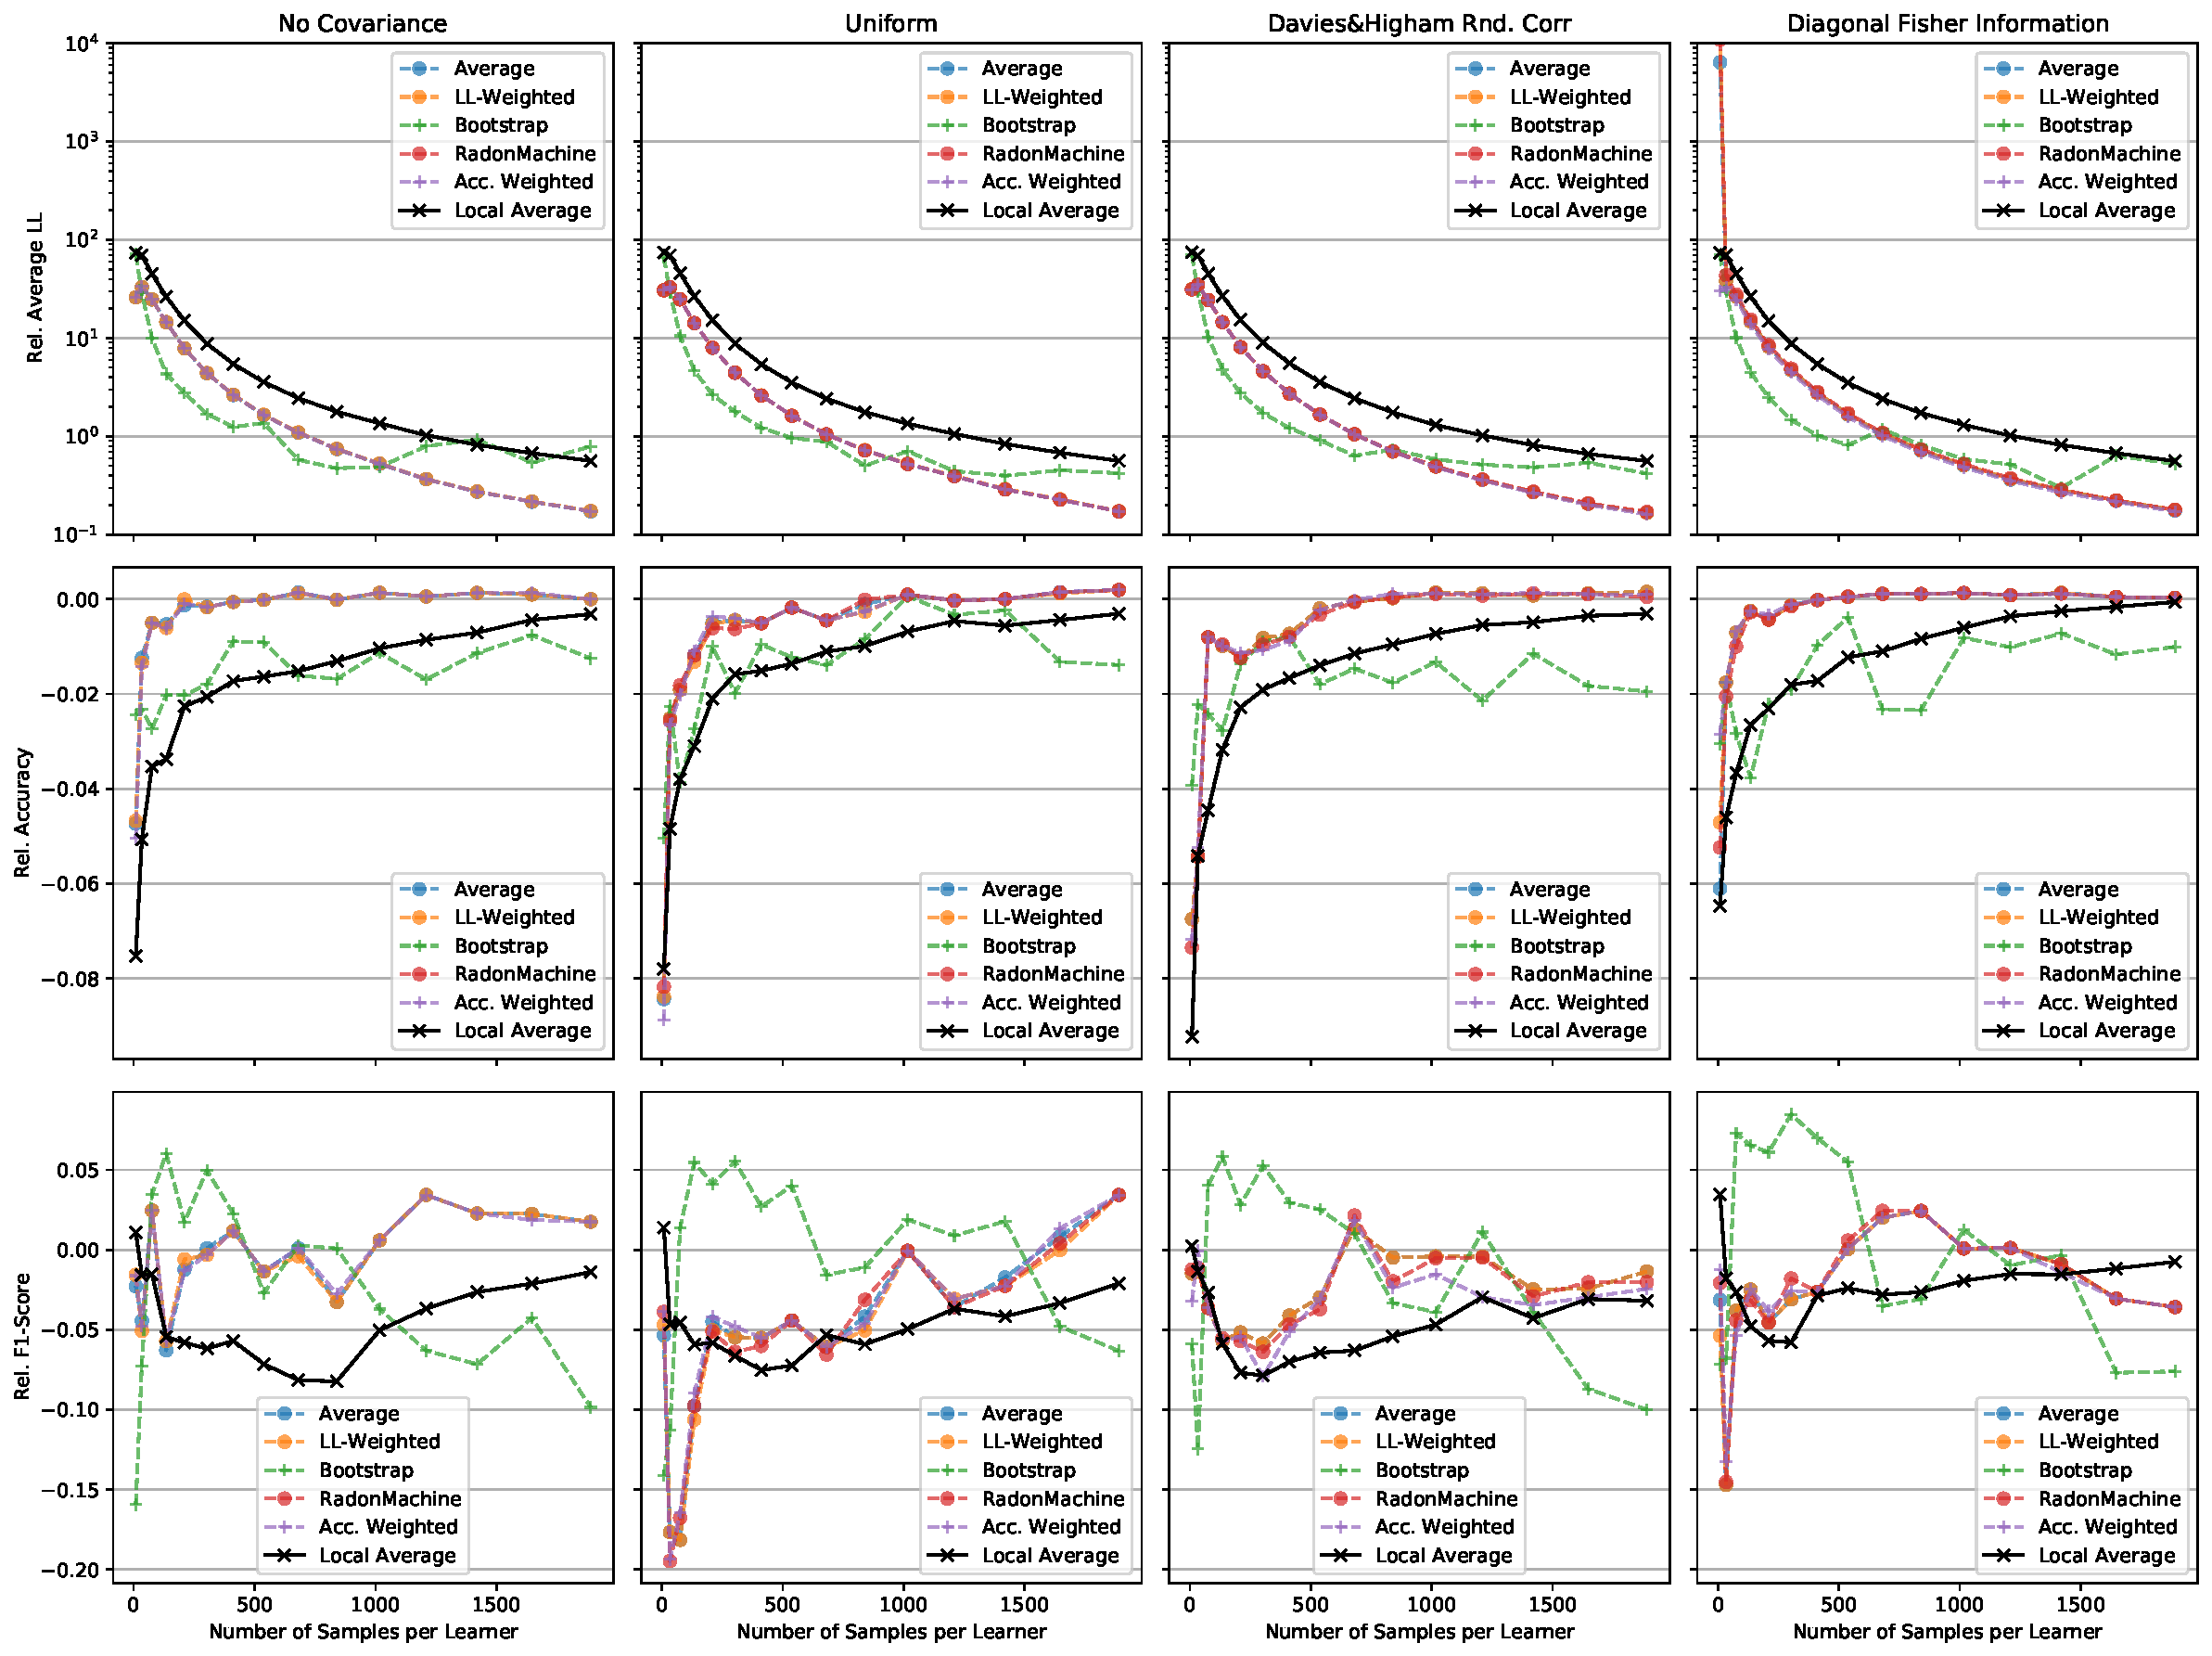
\includegraphics[height=\dimexpr \textheight - 1\baselineskip\relax]{kapitel/figures/susy_None_0.1_neg_relative.pdf}
        \caption[Susy plots without regularization and $\epsilon=0.1$]{Experimental results on the Susy data set for $k=10$ distributed learners. Each plot represents a combination of metric and covariance matrix used for sampling. Values on the x-Axis are the number of samples available on each learner. The top row shows the relative negative average log likelihood $\ell(\tilde{\vect{\theta}}; \mathcal{D}) - \ell(\hat{\vect{\theta}}; \mathcal{D})$  for each aggregate.}
        \label{fig:analysis4}
    \end{figure}
    \end{landscape}
\begin{landscape}
    \begin{figure}
        \centering
        \textbf{Susy, l2 regularization, Bound $\epsilon=0.05$}\par\medskip
        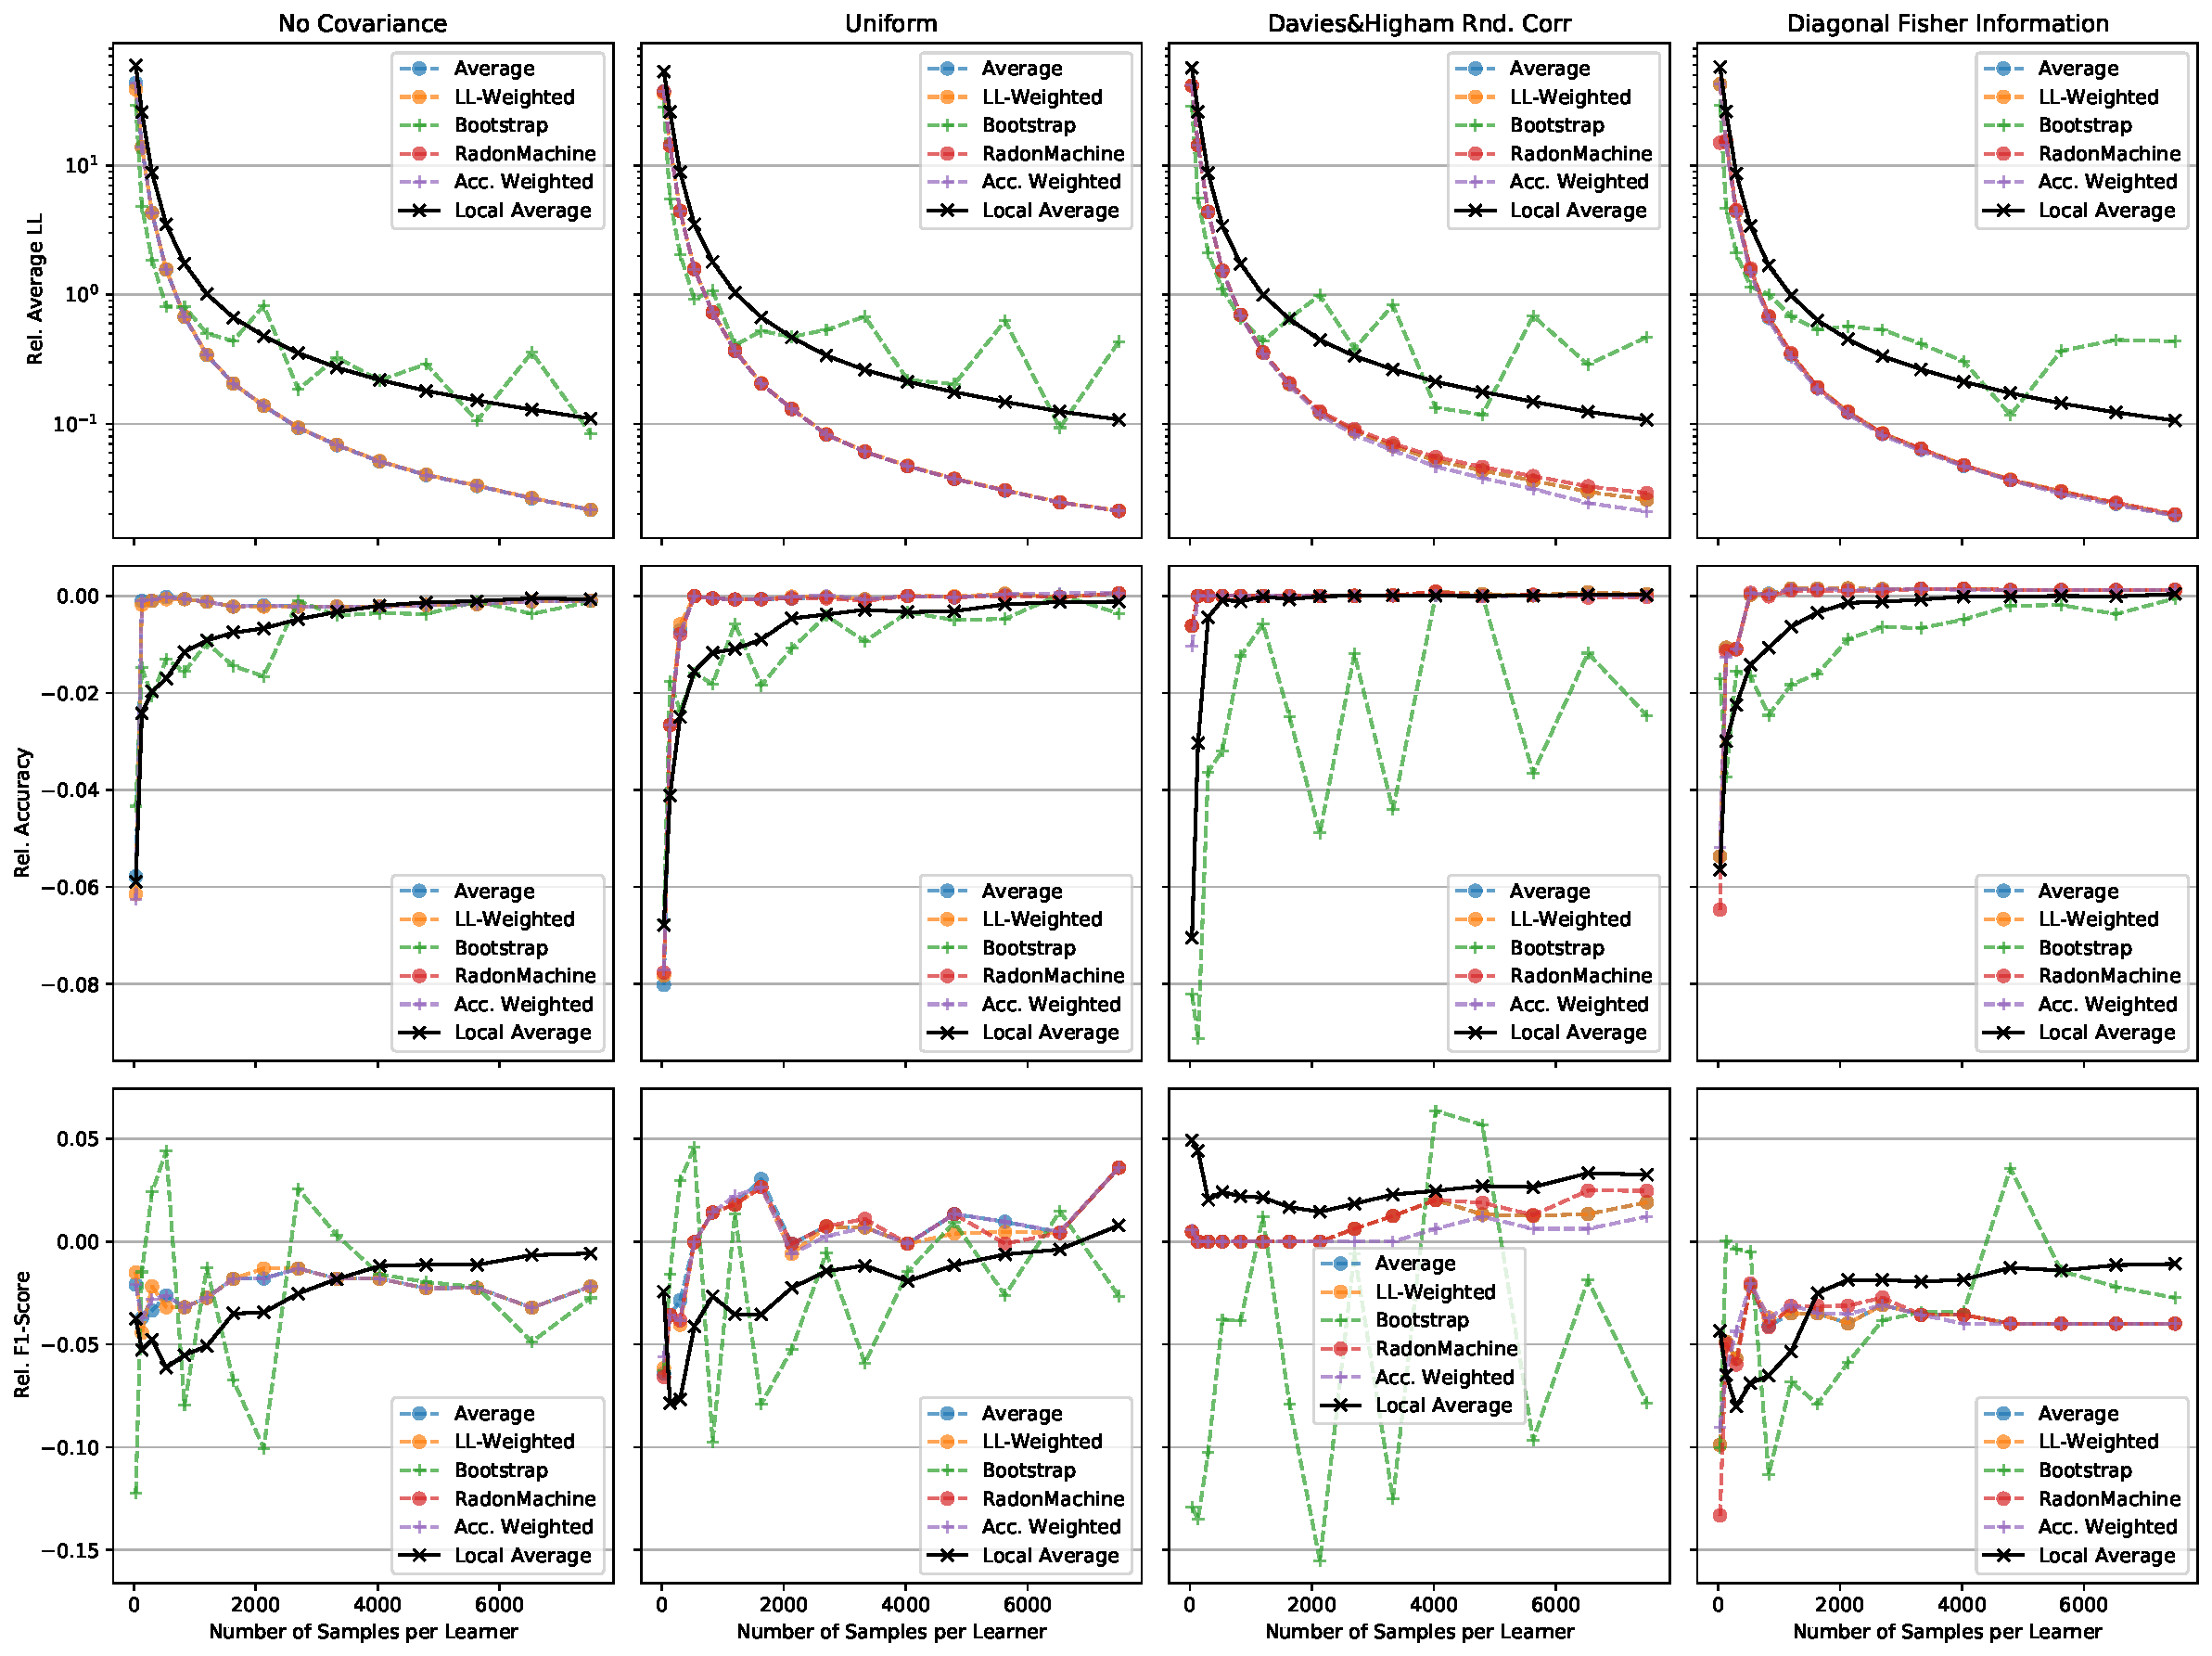
\includegraphics[height=\dimexpr \textheight - 1\baselineskip\relax]{kapitel/figures/susy_l2_0.05_neg_relative.pdf}
        \caption[Susy plots with l2 regularization and $\epsilon=0.05$]{Experimental results on the Susy data set for $k=10$ distributed learners. Each plot represents a combination of metric and covariance matrix used for sampling. Values on the x-Axis are the number of samples available on each learner. The top row shows the relative negative average log likelihood $\ell(\tilde{\vect{\theta}}; \mathcal{D}) - \ell(\hat{\vect{\theta}}; \mathcal{D})$  for each aggregate.}
        \label{fig:analysis1}
    \end{figure}
    \end{landscape}
    \begin{landscape}
    \begin{figure}
        \centering
        \textbf{Covertype, l2 regularization, Bound $\epsilon=0.05$}\par\medskip
        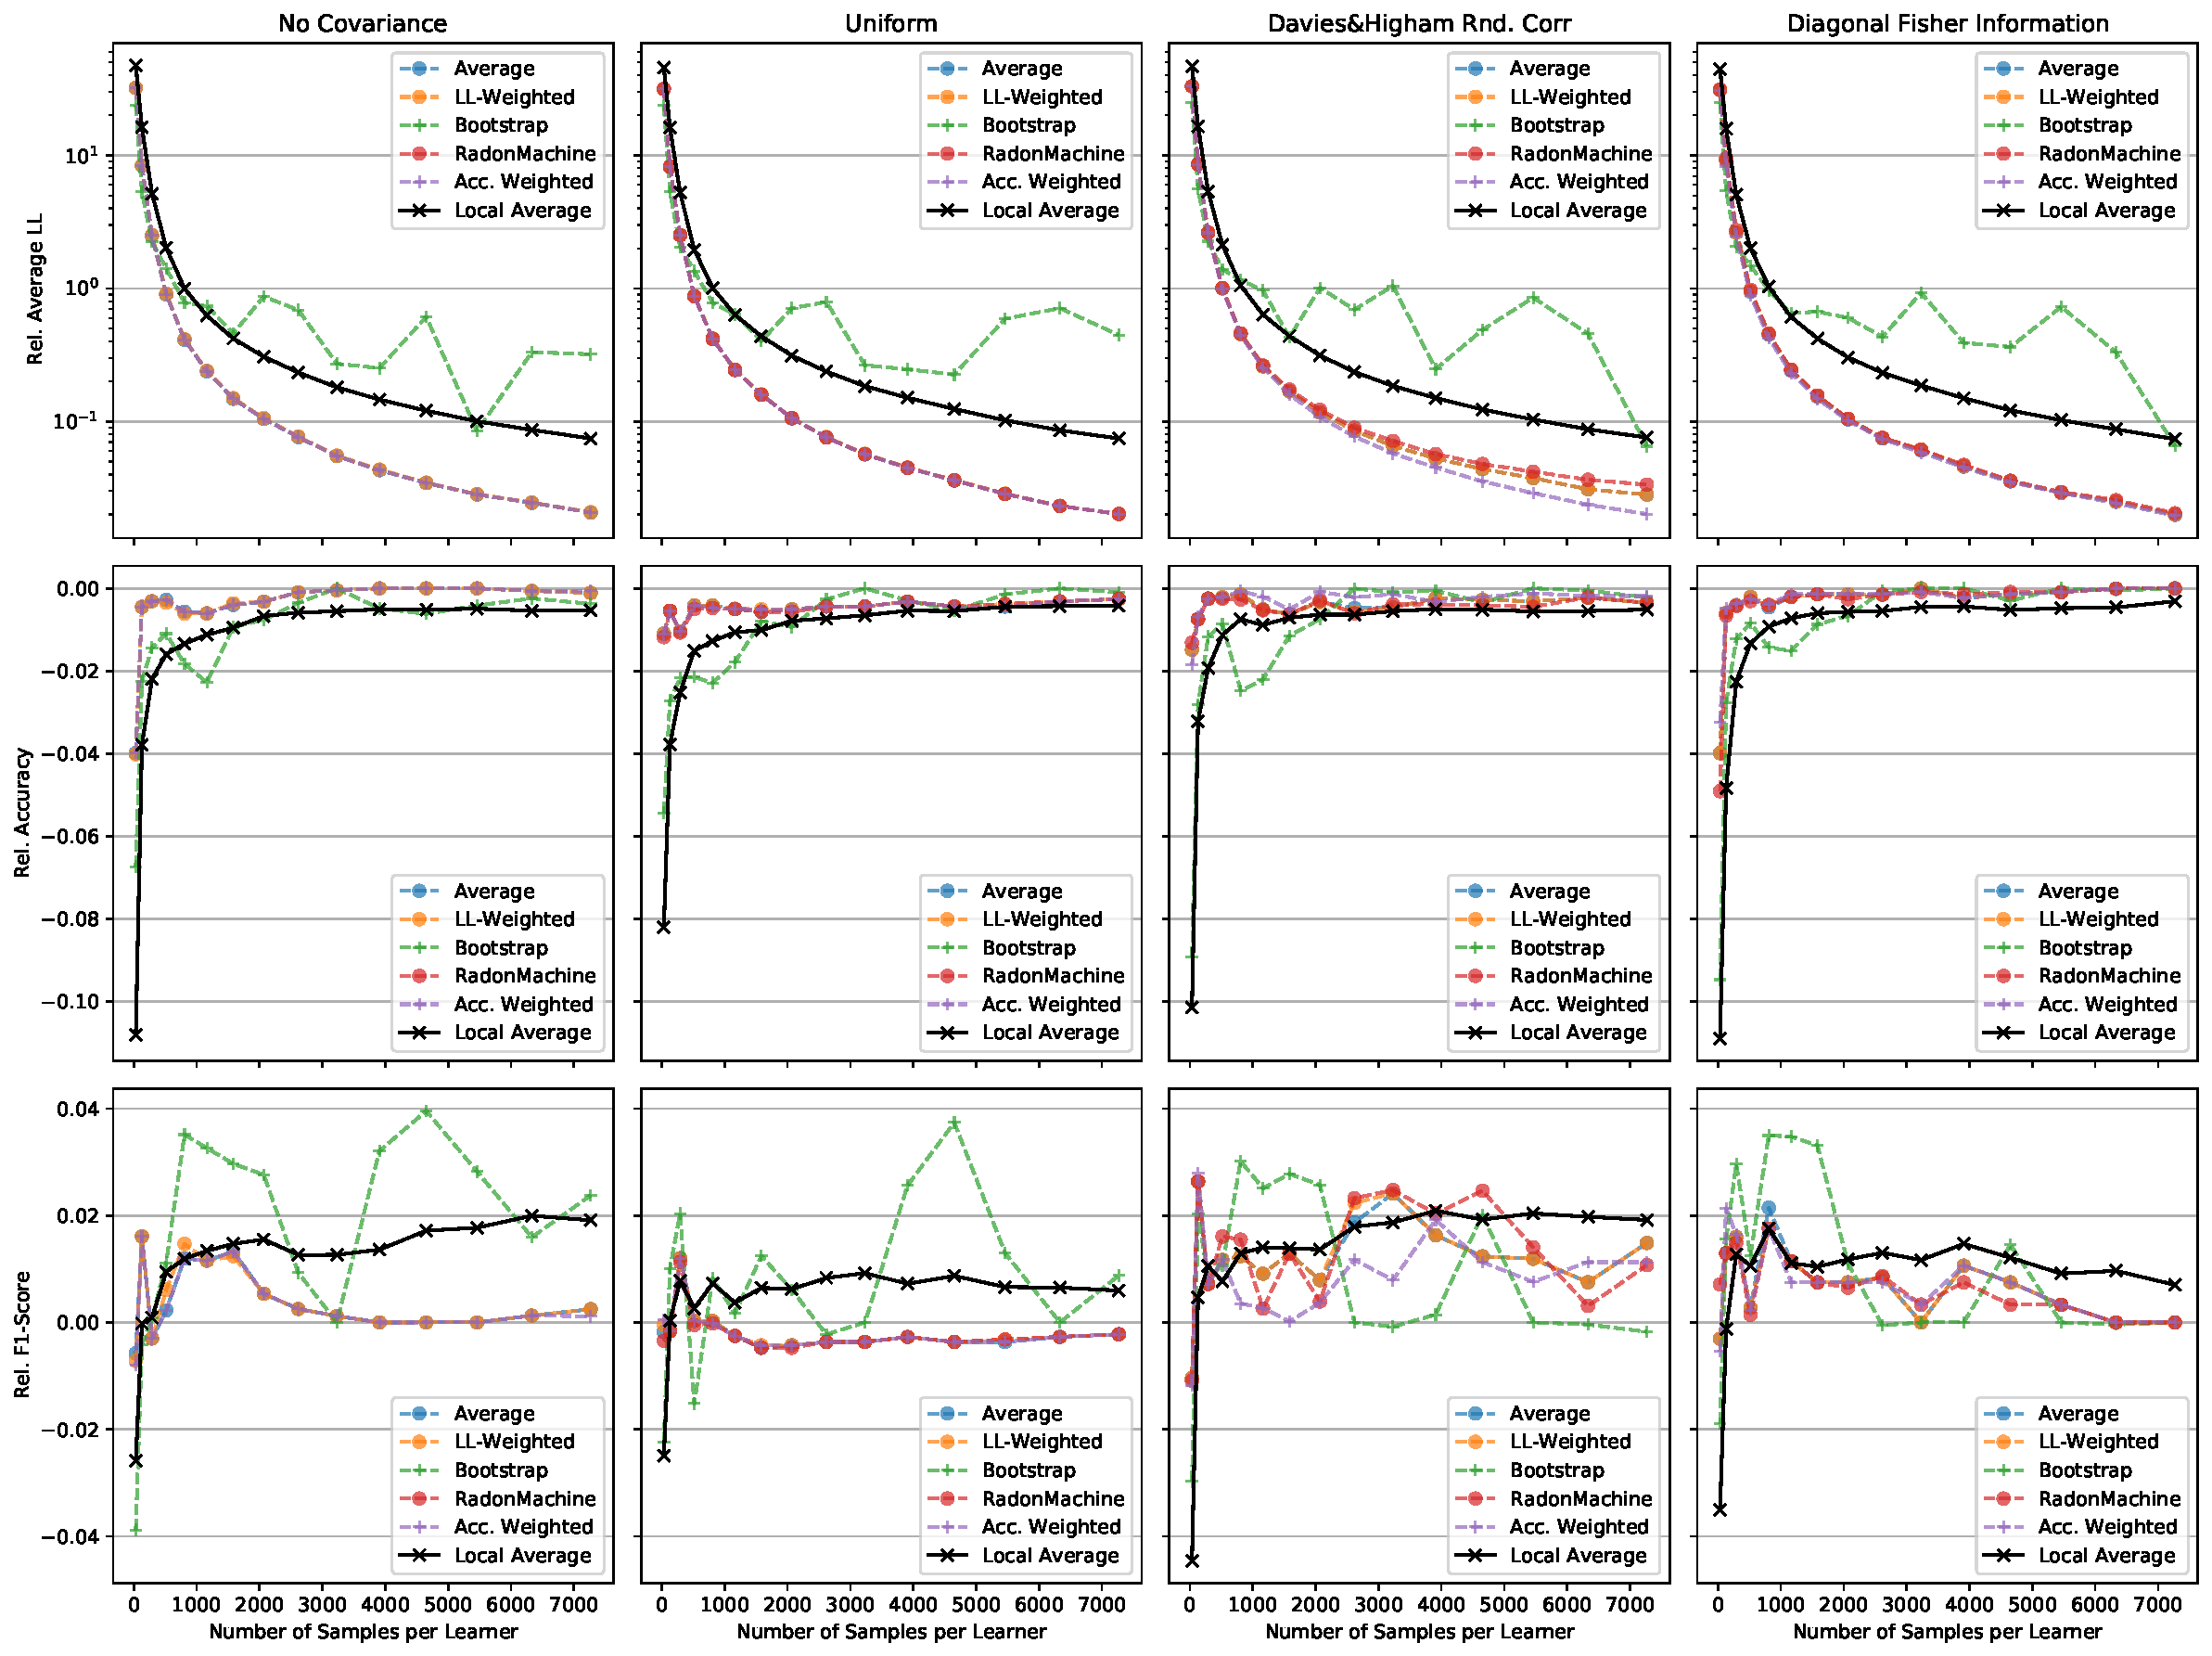
\includegraphics[height=\dimexpr \textheight - 1\baselineskip\relax]{kapitel/figures/covertype_l2_0.05_neg_relative.pdf}
        \caption[Covertype plots with l2 regularization and $\epsilon=0.05$]{Experimental results on the Covertype data set for $k=10$ distributed learners. Each plot represents a combination of metric and covariance matrix used for sampling. Values on the x-Axis are the number of samples available on each learner. The top row shows the negative average log likelihood $\ell(\tilde{\vect{\theta}}; \mathcal{D})$ for each aggregate.}
        \label{fig:analysis2}
    \end{figure}
    \end{landscape}
    \begin{landscape}
        \begin{figure}
            \centering
            \textbf{Dota2, l2 regularization, Bound $\epsilon=0.05$}\par\medskip
            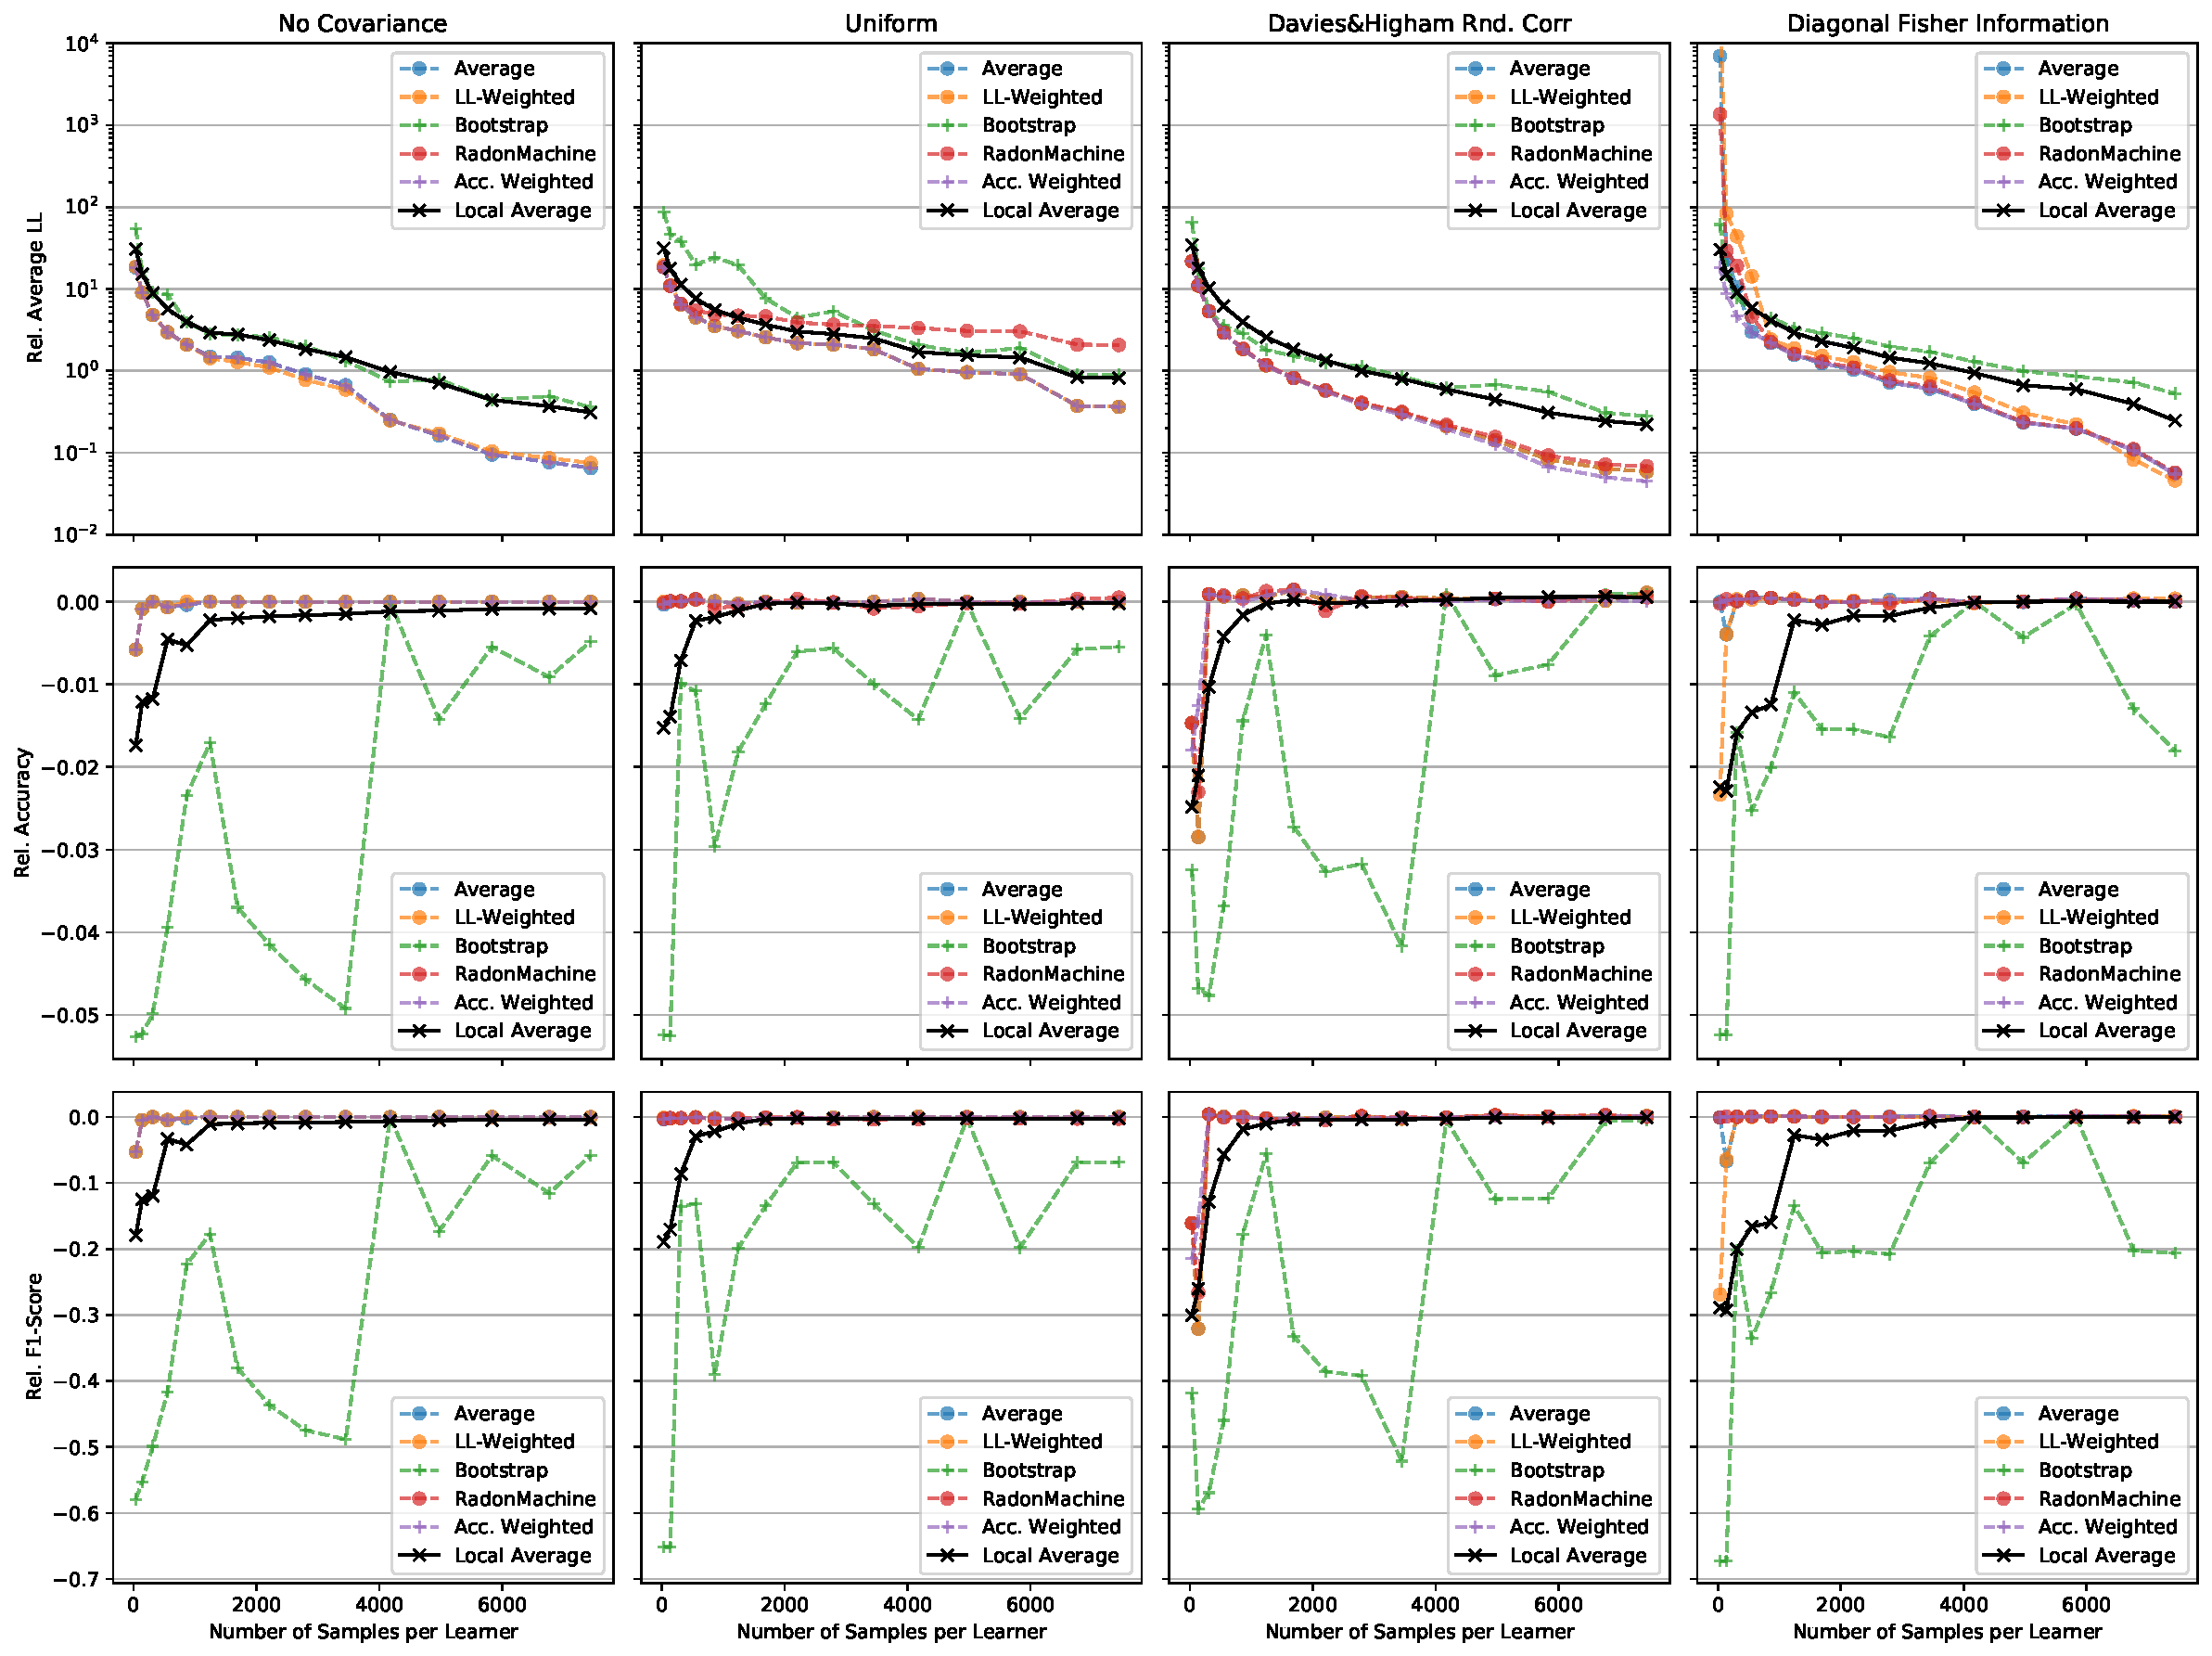
\includegraphics[height=\dimexpr \textheight - 1\baselineskip\relax]{kapitel/figures/dota2_l2_0.05_neg_relative.pdf}
            \caption[Dota2 plots with l2 regularization and $\epsilon=0.05$]{Experimental results on the Dota2 data set for $k=10$ distributed learners. Each plot represents a combination of metric and covariance matrix used for sampling. Values on the x-Axis are the number of samples available on each learner. The top row shows the negative average log likelihood $\ell(\tilde{\vect{\theta}}; \mathcal{D})$ for each aggregate.}
            \label{fig:analysis3}
        \end{figure}
    \end{landscape}

Recall that we compute the relative likelihood (\autoref{eq:dist_ll}) \wrt the likelihood obtained form the baseline model, which had access to the full training data.
All values shown are the average over the cross-validation splits.

The local model's relative likelihood, accuracy, and F1-Score show the average from all $k=10$ distributed learners.
We further visually distinguish between aggregators using additional parameter vectors obtained from sampling, denoted by the circle("o") markers and aggregators that did not use additional parameter vectors with plus ("+") markers.

\paragraph*{Likelihood}
Each plot shows the relative likelihood for the aggregates and local models.
The relative likelihood was computed \wrt the full training set and shifted by the negative average likelihood of the baseline model.
Therefore, a relative likelihood of zero implies that for some other model, it is as good as the baseline.

The relative likelihood steadily decreases towards zero, i.e., the aggregates properly converge towards the baseline model.
We observe that, on average, all aggregation methods, except for the bootstrap aggregation, consistently outperform the local models. 
Only when using the diagonal Fisher information to sample additional parameter vectors from unregularized models (e.g., \autoref{fig:analysis3}), we obtain aggregates that are initially worse than the local learners.
We further notice that all learners consistently converge towards the baseline likelihood being as close as $d_{\ell} = 0.1$ for the larger bound $\epsilon = 0.1$ and for a smaller bound with $\epsilon = 0.05$ up to $d_{\ell} < 0.1$.
%TODO !!!!!
All aggregates converge equally fast towards the baseline likelihood, while generally outperforming the local models.
The bootstrap aggregator's likelihood initially converges faster when compared to the other aggregation mechanisms. 
The rate of convergence, however, tends to decrease with increasing sample size, while ultimately performing poorly when close to the baseline likelihood.
%TODO !!!!!

Interestingly, in the first few iterations, the relative likelihood and accuracy of the aggregates provide the most gain towards the baseline model. 
Later on, aggregates and local models become increasingly similar since aggregates, and local models both converge. 

Overall, most aggregates perform equally well, considering convergence towards the baseline likelihood.
Initially, the bootstrap aggregation provides the best aggregates in terms of the likelihood, while the accuracy-weighted aggregate slightly outpaces the other aggregates when the number of samples increases.

\paragraph*{Accuracy\& F1 Score}
The second and third-row show accuracy and F1-score for all aggregates and local models relative to the baseline score.
Baseline accuracy, for Susy heavily depends on the splits and ranges between 60\% - 70\%, while models trained on Covertype achieve approximately 70\% classification accuracy and 55\% on Dota2.
We observe that the aggregates' and local models' accuracy converges early, with the aggregators typically converging faster.
We observed an exceptionally fast convergence \wrt accuracy in \autoref{fig:analysis4}, while the local models did not reach the aggregator accuracy.
The goal of the aggregation is to match the baseline models as close as possible.
The aggregate models perform slightly better, notably in the early stages, where the most accuracy is gained on the local models. 
Later on, we do not see much of an increase in performance as local models and aggregates are very close to the baseline likelihood and accuracy.

The F1-Score provides a better metric for the classifier performance in a multi-class setting. 
Here we see, that aggregates tend to fall off slightly when compared to the local models.

Overall, the performance in terms of accuracy and F1-Score is comparable to the global model, while only having seen a fraction of the data.
Model aggregation leads to a performance increase in most cases, while no aggregate has a clear advantage against the others.

\paragraph*{Influence of Sampling}
We can interpret the variance applied to parameter sampling as a measure of uncertainty. 
With increasing sample size $n$ the precision increases and in turn the variance decreases as $\Sigma = (1/n\cdot i(\vect{\theta}))$ when sampling from the diagonal Fisher information.
Having observed less data, we are more uncertain about the actual parameters from distributed learners, while with an increasing number of samples, the variance decreases.
We notably observe this property in \autoref{fig:analysis3}, where the initial aggregates perform worse than the local models.
Here, the number of samples used for aggregation is not sufficient to counteract the high initial variance.
Once we pass a threshold of around $n=500$  samples on each learner, the aggregates' performance increases, crossing the local model's likelihood.

All in all, the aggregates converge faster than the local models and thus contribute to an overall improvement in likelihood and accuracy.


\section{Discussion}
\label{sec:results}

Our findings suggest that probabilistic graphical models trained in a federated system generally benefit from model parameter aggregation, especially when data is limited.
The choice of the aggregation method did not significantly affect the quality of the solution, and sampling parameter vectors was a convenient method for using Radon machines.
Furthermore, the bootstrap aggregation outperforms all other methods early on, implying that bootstrapping samples helps achieving faster convergence until the number of samples increases, where the convergence rate drops off.

The empirical results suggest that the simple independence structure causes fast convergence and high similarity between aggregates.
Since the models on distributed learners converge almost as fast as the aggregates, we quickly reach the pseudo-asymptotic case, where most models are approximately equal. 

Radon Machines, for example, are used to compute the center point or center of mass, which is a generalized approach for computing the geometric median.
While the geometric median, does generally not coincide with the maximum likelihood estimator of a normal distribution~\cite{small1990survey}, our experiments suggest that they are at least similar.
The accuracy-weighted aggregator is better able to balance worse-performing models by assigning lower weights to these models, resulting in a slightly more stable aggregate.
While this works on distributed models with a low amount of samples, the aggregates and local models do ultimately converge fast due to the independence graph's tree characteristic.
Thus, the aggregators do improve the likelihood early by including prior information about the parameters.

The noise introduced by sampling from the normal distribution reflects the actual uncertainty of the sample distribution.
While the variance $1/(n \cdot \vect{\theta}^i)$ does decrease over time, it still introduced a new error when sampling models.

In this case, we have created d+2 models from 10 models, which is an increase of 1500-2500 models based on the number of parameters.
However, when we have a large number of models and only require some additional parameters to increase the aggregation depth of the radon machines, we can diversify the set of models by sampling.

All in all, the convergence interval is with $n=250$ so small that significant improvements can only be observed in the first few iterations.

\paragraph*{Do local models benefit from aggregation?}
Especially in the early stages, where data is scarce, the aggregates severely outperform the distributed learners.
Once the number of samples on the distributed learners increases, the performance gap between distributed learners and aggregates diminishes, with aggregates still having a slight edge in terms of likelihood and accuracy.

\paragraph*{How do aggregation methods compare to each other?}
While the aggregates perform better than the models on distributed learners, no method was able to outperform the others when evaluating at the point of convergence.
However, the bootstrap aggregation was initially faster to converge but did not come as close to the baseline as the other aggregations.
Here, increasing the number of iterations for the Gibbs sampler or merely increasing the number of samples generated may improve upon these results, this however, has implications for runtime.
The Tables\ref{tab:1} and \ref{tab:12} exhibit a quantitative analysis of the relative likelihood.
\autoref{tab:1} shows the relative likelihood without regularizer and without generating additional parameter vectors.
The bootstrap aggregation converges faster, while the accuracy-weighted aggregate performs better after having observed $n=397$ samples.
\autoref{tab:12} shows the relative likelihood with parameter vector sampling from the diagonal Fisher information. 
We compare the aggregates using sample parameter vectors and the aggregates not using them separately.
Here, the arithmetic mean performs the best out of the three methods, while again, the bootstrap aggregation is initially better than the accuracy-weighted aggregation.


\paragraph*{Do additional parameter samples affect the aggregate?}
The increased variance led to initially worse aggregates, while overall not improving the final result.
Overall, sampling parameter vectors is useful for enabling aggregation methods such as Radon machines and increasing diversity, i.e., acting as a regularizer for the bias-variance tradeoff.
Investigating the Fisher information matrix to find parameters with high variance may be an alternative to sampling parameter vectors.

\paragraph*{How do aggregates perform when compared to the baseline?}
The likelihood is an indicator of model performance but does not directly translate to accuracy and F1-score.
Compared to the baseline, the aggregates were close, but in the end, could not fully capture the baseline distribution.
Our experiments suggest that he bootstrap aggregation converges faster, but not correctly towards the baseline, such that the local models perform better with increasing sample size.

\begin{table}
\centering
\caption[Covertype relative likelihood with $\epsilon=0.1$, without regularization]{Relative Likelihood when compared to the baseline likelihood on the test split. This table shows the results for  Covertype without sampling additional parameter vectors with epsilon $\epsilon= 0.1$, without regularization. The best performing aggregate is highlighted with bold-faced letters. The bootstrap aggregation performs well early on, while later dropping off when compared to the other aggregates.}
\label{tab:1}
\resizebox{\textwidth}{!}{%
\begin{tabular}{|l||r|rrrrr|}
\toprule
{} &  Local Average &  Average &  RadonMachine &  LL-Weighted &  Bootstrap &  Acc. Weighted \\
Num Samples &                &          &               &              &            &                \\
\midrule
9      &          65.82 &    \textbf{27.10} &           --- &        26.79 &      55.48 &          27.14 \\
33     &          48.63 &    \textbf{20.10} &           --- &        20.14 &      20.40 &          20.11 \\
73     &          29.23 &    13.95 &           --- &        14.01 &       \textbf{9.52} &          13.96 \\
130    &          16.51 &     7.99 &           --- &         8.02 &       \textbf{4.17} &           7.99 \\
203    &           9.21 &     4.65 &           --- &         4.67 &       \textbf{2.64} &           4.65 \\
292    &           5.35 &     2.60 &           --- &         2.62 &       \textbf{1.97} &           2.60 \\
397    &           3.10 &     1.48 &           --- &         1.48 &       1.65 &           \textbf{1.48} \\
519    &           2.03 &     0.90 &           --- &         0.91 &       2.01 &           \textbf{0.90} \\
657    &           1.40 &     0.60 &           --- &         0.61 &       1.26 &           \textbf{0.60} \\
810    &           1.04 &     0.43 &           --- &         0.43 &       0.75 &           \textbf{0.43} \\
981    &           0.78 &     0.30 &           --- &         0.30 &       0.79 &           \textbf{0.30} \\
1167   &           0.62 &     0.23 &           --- &         0.23 &       0.86 &           \textbf{0.23} \\
1369   &           0.54 &     0.20 &           --- &         0.20 &       0.44 &           \textbf{0.20} \\
1588   &           0.45 &     0.16 &           --- &         0.16 &       1.09 &           \textbf{0.16} \\
1823   &           0.38 &     0.13 &           --- &         0.13 &       0.50 &           \textbf{0.13} \\
\bottomrule
\end{tabular}%
}
\end{table}

\begin{table}
\centering
\caption[Susy relative likelihood with $\epsilon=0.1$, without regularization]{Relative Likelihood when compared to the baseline likelihood on the full training split. This table shows the results on the Susy data set using additional parameter vectors sampled with the diagonal Fisher information. The best performing aggregate is highlighted with bold-faced letters.. Note that we do not directly compare the three aggregation methods to the other two on the right, as the rightmost aggregates do not use the additional samples. The bootstrap aggregation performs well early on, while later dropping off when compared to the other aggregates.}
\label{tab:12}
\resizebox{\textwidth}{!}{%
\begin{tabular}{|l||r|rrr||rr|}
\toprule
{} &  Local Average &  Average &  RadonMachine &  LL-Weighted &  Bootstrap &  Acc. Weighted \\
Num Samples &                &          &               &              &            &                \\
\midrule
9      &          \textbf{74.34} &  6390.09 &      10844.96 &     12381.15 &      70.65 &          \textbf{30.35} \\
34     &          70.12 &    \textbf{38.21} &         43.66 &        38.21 &      \textbf{29.49} &          32.67 \\
76     &          45.28 &    \textbf{26.47} &         27.67 &        26.47 &      \textbf{10.10} &          24.55 \\
135    &          26.41 &    \textbf{14.82} &         15.45 &        14.82 &      \textbf{ 4.50} &          13.92 \\
210    &          14.95 &    \textbf{ 8.14} &          8.48 &         8.14 &      \textbf{ 2.48} &           7.67 \\
303    &           8.78 &    \textbf{ 4.73} &          4.90 &         4.74 &      \textbf{ 1.47} &           4.46 \\
412    &           5.44 &    \textbf{ 2.77} &          2.83 &         2.77 &      \textbf{ 1.02} &           2.62 \\
538    &           3.50 &    \textbf{ 1.67} &          1.72 &         1.68 &       0.82 &           \textbf{1.58} \\
681    &           2.40 &    \textbf{ 1.06} &          1.08 &         1.07 &       1.17 &           \textbf{1.01} \\
840    &           1.73 &    \textbf{ 0.72} &          0.73 &         0.73 &       0.82 &           \textbf{0.69} \\
1017   &           1.31 &    \textbf{ 0.51} &          0.52 &         0.51 &       0.59 &           \textbf{0.48} \\
1210   &           1.02 &    \textbf{ 0.36} &          0.38 &         0.37 &       0.52 &           \textbf{0.35} \\
1420   &           0.82 &    \textbf{ 0.28} &          0.29 &         0.28 &       0.30 &           \textbf{0.27} \\
1647   &           0.68 &    \textbf{ 0.22} &          0.22 &         0.22 &       0.64 &           \textbf{0.22} \\
1890   &           0.56 &    \textbf{ 0.18} &          0.18 &         0.18 &       0.52 &           \textbf{0.17} \\
\bottomrule
\end{tabular}%
}
\end{table}

%\begin{table}
%    \centering
%    \caption{Relative Likelihood when compared to the baseline likelihood on the test split. This table shows the results for Covertype using fish sampling with epsilon  0.1 and  default regularization.}
%    \label{tab:0}
%    \resizebox{0.7\columnwidth}{!}{%
%    \begin{tabular}{|l||r|rrr|rr|}
%    \toprule
%    \bottomrule
%    \end{tabular}%
%    }
%    \end{table}
   